\documentclass[]{article}
\usepackage[spanish.mexico]{babel}
\usepackage[T1]{fontenc}
\usepackage[utf8]{inputenc}
%\usepackage{lmodern}
\usepackage[a4paper]{geometry}

%Graficos e imagenes
\usepackage{graphicx}
%\graphicspath{ Imagenes/ }

\usepackage{cite}

%Grafico de barras
%\usepackage{pgfplots}


\usepackage{tikz}
\usepackage[american voltages, american currents,siunitx]{circuitikz}

%\title{Proyecto de Optimización de Energía}
%\author{Pablo Vivar Colina}
%\date{Mayo 2018}



\begin{document}
	
%\usepackage[top=2cm,bottom=2cm,left=1cm,right=1cm]{geometry}


\begin{titlepage}
     \begin{center}
	
\includegraphics[width=0.09\textwidth]{UNAM}\Large Universidad Nacional Autónoma de México
        	
\includegraphics[width=0.09\textwidth]{FI}\\[1cm]
        \Large Facultad de Ingeniería\\[1cm]
       % \Large División de Ciencias Básicas\\[1cm]
         \Large Laboratorio de Fundamentos de Control(6655)\\[1cm]
         %la clave antes era:4314
         \footnotesize Profesor: Salcedo Ubilla María Leonor Ing.\\[1cm]
        \footnotesize Semestre 2019-1\\[1cm]
        
       

        \Large Práctica No. 1\\[1cm]
        
           

\Large Introdcción MATLAB
        
         %Texto a la derecha
          \begin{flushright}
\footnotesize  Grupo 2\\[0.5cm]
\footnotesize Brigada: 4\\[0.5cm]
\footnotesize Rodrigo Adrián Martínez López\\[0.5cm]
\footnotesize Vivar Colina Pablo\\[0.5cm]
 \end{flushright}
    %Texto a la izquierda
          \begin{flushleft}
        \footnotesize Ciudad Universitaria Agosto de 2018.\\
          \end{flushleft}
         
          
        %\vfill
        %\today
   \end{center}
\end{titlepage}
 %agregar portada

%\maketitle

\tableofcontents  % Write out the Table of Contents

%\listoffigures  % Write out the List of Figures

\section{Resumen}

\section{Introducción}


\subsection{NI ELVIS}

Para crear una aplicación completa de NI ELVIS, explore otras soluciones de laboratorio para NI ELVIS.\\

Proporciona una experiencia de aprendizaje basada en proyectos, usando medidas en línea y diseño práctico y embebido.\\

El NI Educational Laboratory Virtual Instrumentation Suite (NI ELVIS) es un dispositivo modular de laboratorio educativo de ingeniería desarrollado específicamente para la academia. Con este enfoque práctico, los profesores pueden ayudar a los estudiantes a aprender habilidades de ingeniería prácticas y experimentales. NI ELVIS incluye un osciloscopio, multímetro digital, generador de funciones, fuente de alimentación variable, analizador de Bode y otros instrumentos comunes de laboratorio. Puede conectar una PC al NI ELVIS usando USB y desarrollar circuitos en su protoboard desmontable.\cite{NationalInstruments2018}\\


\section{Objetivos}

\subsection{Objetivos generales}


\begin{itemize}
	\item El estudiante experimentará la aplicación física de un controlador PID, basado en una computadora personal y el software LabView, y verificará la salida del proceso físico con los resultados de la simulación correspondiente.
	\end{itemize}

\subsection{Objetivos específicos}

\begin{itemize}
	\item El estudiante aplicará su conocimiento de un controlador PID, para entender de manera práctica los efectos de cada acción de la ley de control, en base al algoritmo de la teoría clásica de control.

  \item El estudiante entenderá y se familiarizará con un sistema de control digital PID que en base al tiempo de muestreo asociado y la programación de una aplicación de Instrumentación Virtual, comprenderá lo que significa la sintonización para el sistema de control.

\item El estudiante podrá ser capaz de realizar la sintonización para una planta de manera experimental y que en base al método de Oscilaciones Amortiguadas, podrá comprobar que los valores para cada parámetro del controlador PID son los adecuados para obtener respuestas deseadas en el sistema de control.

 \item El estudiante verificará de manera práctica que un controlador robusto tiene un desempeño eficiente con corrección de errores a pesar de perturbaciones y cambios de carga.
	\end{itemize}


\section{Materiales y métodos}

 En esta práctica, el algoritmo de control corresponde a la acción PID realizada por medio del software LabView, el cual provee un ambiente gráfico de programación y operación, en lo que se conoce como un instrumento o controlador virtual. La construcción del sistema se muestra en la Figura 2, en donde destaca la tarjeta de adquisición de datos de Nacional Instruments PCI-6221M , las cuales disponen de 16 canales A/D de entrada analógica de voltaje, en el intervalo de -10 a 10 volts y dos canales D/A de salida digital del mismo rango. \\
		
		El controlador se llama PID Harriot y para operar requiere de elementos de software que ya han sido instalados, el Run time engine de LabView y el driver de la tarjeta de adquisición de datos, para enlazar el hardware con el programa de control.\\

	
\section{Resultados}





\begin{equation}
  \frac{1.42}{s^2+2.42s+1.42}
\end{equation}



\begin{figure}[h!]
	\centering
	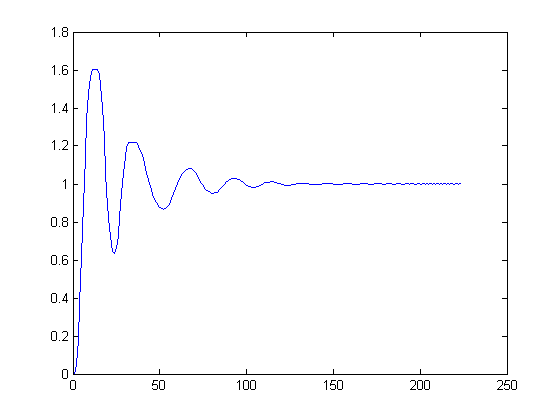
\includegraphics[width=0.6\textwidth]{Imagenes/modelo2Const}
	\caption{Valores de PID Kc=3, Ti=1}
	\label{fig:modeloConst}
\end{figure}

\begin{figure}[h!]
	\centering
	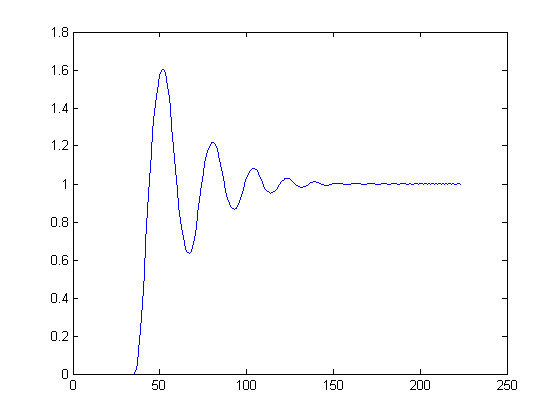
\includegraphics[width=0.6\textwidth]{Imagenes/modeloEscalon}
	\caption{Valores de PID Kc=3, Ti=1}
	\label{fig:modeloEscalon}
\end{figure}

\begin{figure}[h!]
	\centering
	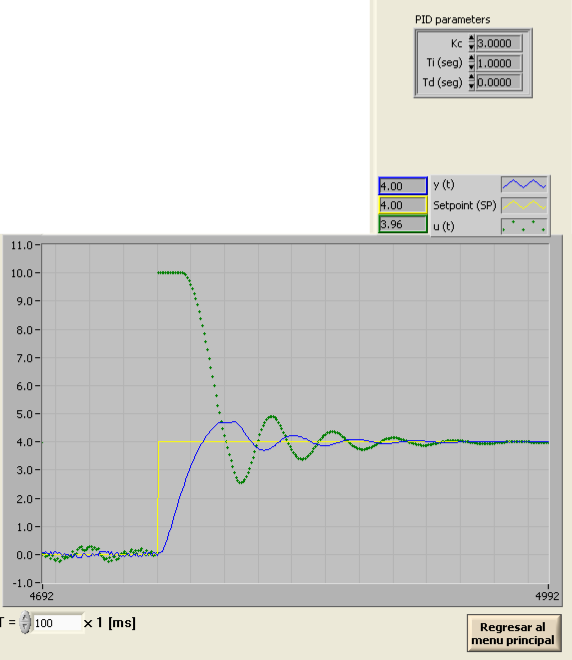
\includegraphics[width=0.6\textwidth]{Imagenes/signalActividad1}
	\caption{Valores de PID Kc=3, Ti=1}
	\label{fig:signalActividad1}
\end{figure}

\begin{figure}[h!]
	\centering
	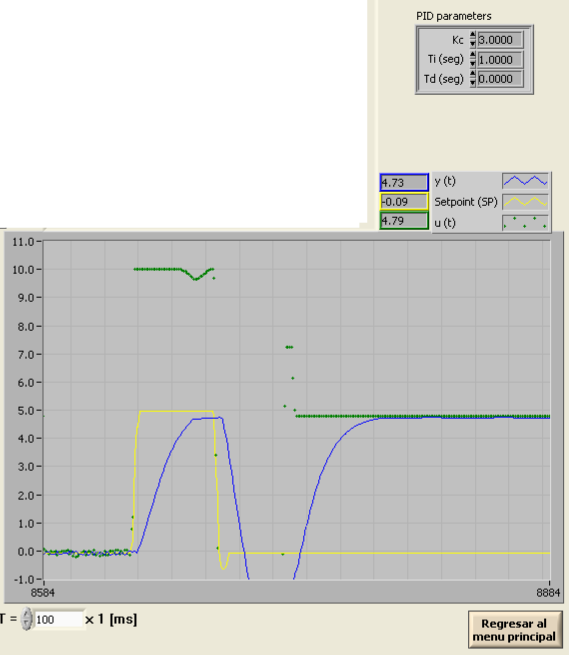
\includegraphics[width=0.6\textwidth]{Imagenes/signalActividad2}
	\caption{Valores de PID Kc=3, Ti=1}
	\label{fig:signalActividad2}
\end{figure}

\begin{figure}[h!]
	\centering
	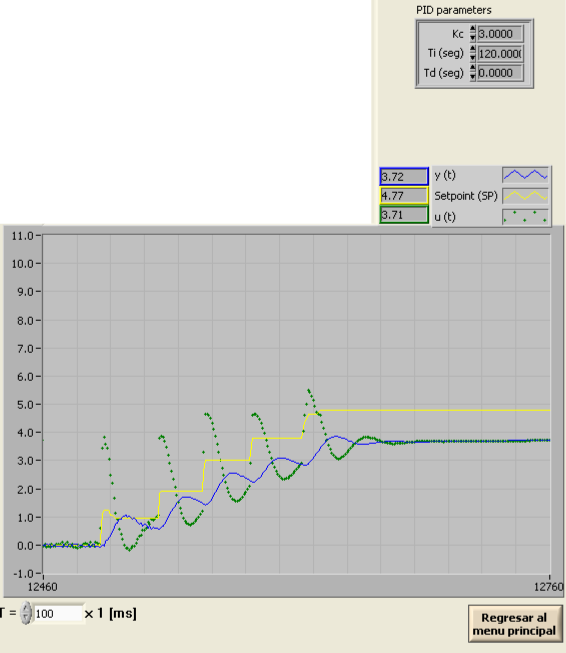
\includegraphics[width=0.6\textwidth]{Imagenes/signalActividad2B}
	\caption{Valores de PID Kc=3, Ti=120}
	\label{fig:signalActividad2B}
\end{figure}


\begin{figure}[h!]
	\centering
	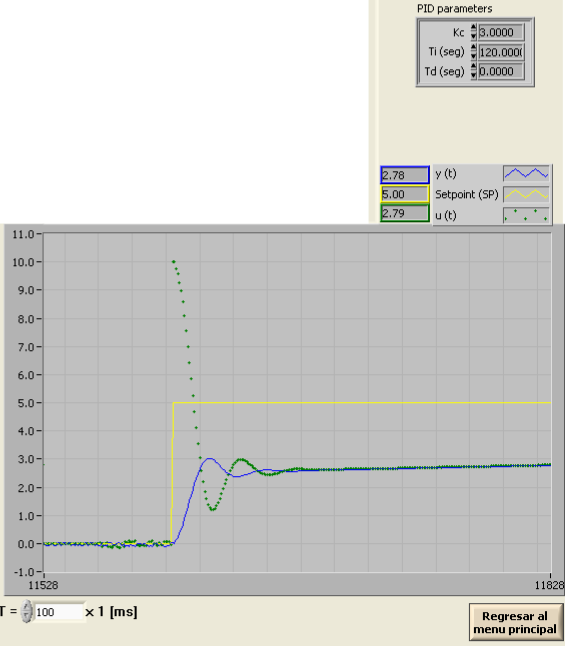
\includegraphics[width=0.6\textwidth]{Imagenes/signalActividad3}
	\caption{Valores de PID Kc=3, Ti=120}
	\label{fig:signalActividad3}
\end{figure}

\begin{figure}[h!]
	\centering
	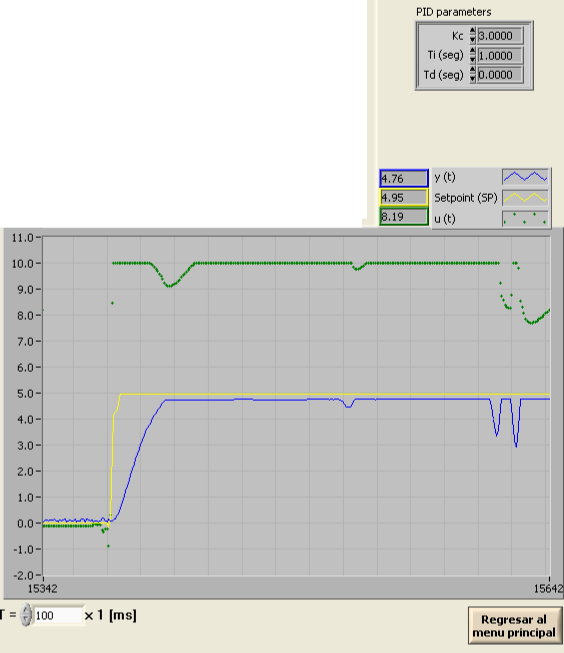
\includegraphics[width=0.6\textwidth]{Imagenes/signalActividad4A}
	\caption{Valores de PID Kc=3, Ti=1}
	\label{fig:signalActividad4A}
\end{figure}

\begin{figure}[h!]
	\centering
	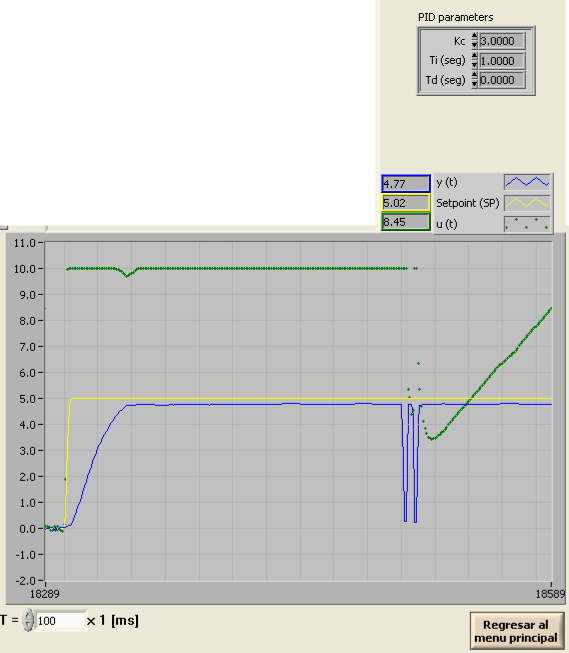
\includegraphics[width=0.6\textwidth]{Imagenes/signalActividad4b}
	\caption{Valores de PID Kc=3, Ti=1}
	\label{fig:signalActividad4b}
\end{figure}

\begin{figure}[h!]
	\centering
	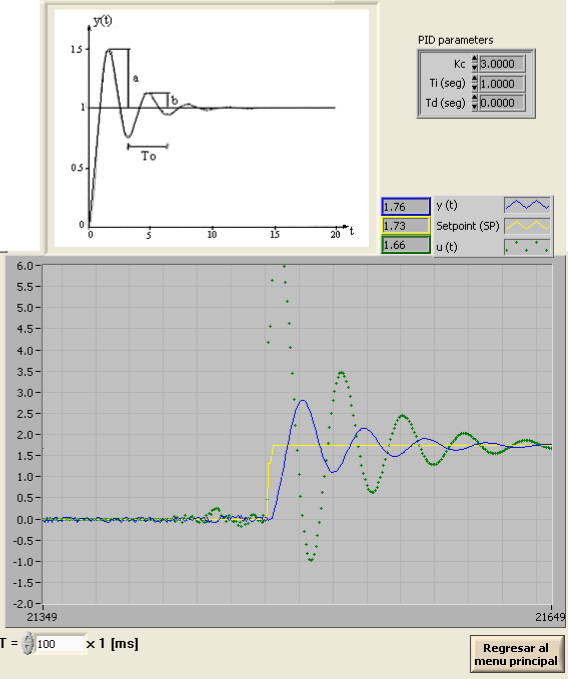
\includegraphics[width=0.6\textwidth]{Imagenes/signalActividad6prueba1}
	\caption{Valores de PID Kc=3, Ti=1}
	\label{fig:signalActividad6prueba1}
\end{figure}

\begin{figure}[h!]
	\centering
	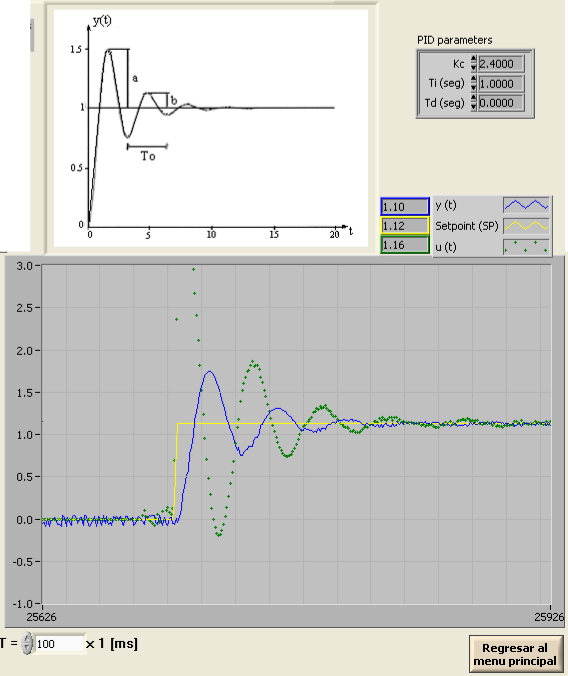
\includegraphics[width=0.6\textwidth]{Imagenes/signalActividad6prueba2}
	\caption{Valores de PID Kc=2.4, Ti=1}
	\label{fig:signalActividad6prueba2}
\end{figure}

\begin{figure}[h!]
	\centering
	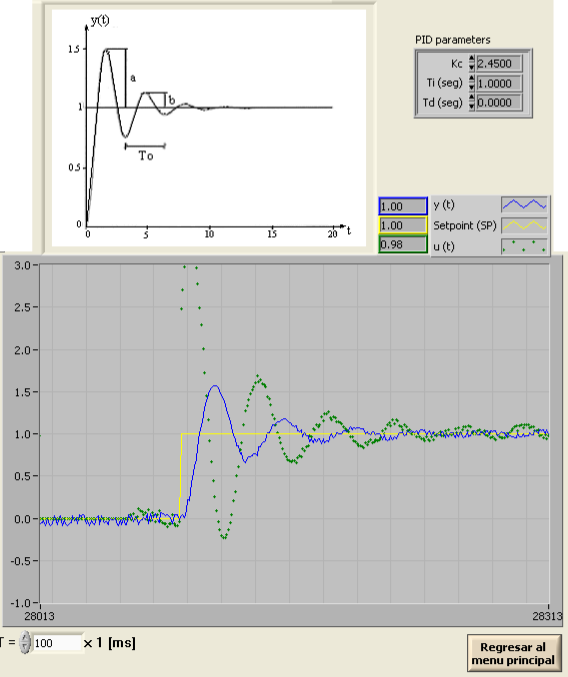
\includegraphics[width=0.6\textwidth]{Imagenes/signalActividad6prueba3}
	\caption{Valores de PID Kc=2.45, Ti=1}
	\label{fig:signalActividad6prueba3}
\end{figure}





\section{Análisis de Resultados}



\section{Conclusiones}


\section{Referencias}

\bibliographystyle{plain}
\bibliography{Referencias.bib}



\end{document}
